\documentclass{article}
\usepackage[margin=1in]{geometry}
\usepackage{amsmath}
\usepackage{amsfonts}
\usepackage{graphicx}
\usepackage{xcolor}
\usepackage{ulem}
\usepackage{comment}
\input{sym}


\title{ECE 498/598 Midterm 2 2023}
\date{Nov 8th, 2023}
\author{Instructor: Vikas Dhiman}

\newtheorem{prob}{Problem}
\newif\ifsol
\soltrue

\ifsol
  \newenvironment{solution}{\emph{Solution:}}{}
\else
  \excludecomment{solution}
\fi


\begin{document}
\maketitle
%$ \hat{\mathbf{w}} = \hat{\mathbf{k}} \times \frac{\mathbf{v}}{\|\mathbf{v}\|} $
%$ \|\hat{\mathbf{w}}\| = \|\hat{\mathbf{k}}\| \|\frac{\mathbf{v}}{\|\mathbf{v}\|}\| \sin(\phi) $. 

\begin{tabular}{p{0.5\linewidth}p{0.5\linewidth}}
  (1) Student name:& Student email: \\
\end{tabular}

\subsubsection*{About the exam}
\begin{enumerate}
  \item There are total 4 problems. You must attempt all 4.
  \item Maximum marks: 50.
  \item Maximum time allotted:  50 min
  \item Calculators are allowed.
  \item One US Letter size or A4 size cheat sheet (both-sides) is allowed.
\end{enumerate}

\begin{prob}
  Find the 4x4 transformation matrix $^1T_0$ that transforms coordinates from coordinate frame 1 to coordinate frame 0 (5 marks).\\
  \includegraphics[width=0.7\linewidth,trim=0 0 0 1in,clip]{./media/transformations.png}
\end{prob}
\begin{solution}
I am going to write transform from frame 1 to frame 0. $^0T_1$
\begin{align}
  ^0T_1 = \begin{bmatrix}
    1 & 0 & 0 & -3.5\\
    0 & -1 & 0 & 3 \\
    0 & 0 & -1 & 1\\
    0 & 0 & 0 & 1
  \end{bmatrix}
\end{align}
The rotation matrix is obtained by writing the basis vectors of the destination coordinate system in the source coordinate system.

\end{solution}
\newpage
.
\newpage

\begin{prob}
  Consider a coordinate system OUVW whose ordered set of basis vectors given by
  $\bfu = [3/7, 2/7, 6/7]^\top$, $\bfv = [2/7, 6/7, 3/7]^\top$ and $\bfw = [4,
  5, 6]^\top$.
  Another coordinate system OXYZ whose order set of basis vectors is, $\bfx =
  [2/7, 6/7, -3/7]^\top$, $\bfy = [-6/7, 3/7, 2/7]^\top$ and $\bfz = [3/7, 2/7, 6/7]^\top$.
  Find the rotation matrix $^{ouvw}R_{oxyz}$ that converts coordinates from frame OXYZ to frame OUVW. (10 marks)
\end{prob}
\begin{solution}

Let OPQR be the coordinate system in which the coordinates of basis vectors are specified.
\begin{align}
  ^{OPQR}R_{OUVW} &= \begin{bmatrix}
    | & | & | \\
    \bfu & \bfv & \bfw \\
    | & | & | \\
  \end{bmatrix}
    = \begin{bmatrix}
    3/7 & 2/7 & 4 \\
    2/7 & 6/7 & 5  \\
    6/7 & 3/7 & 6 \\
  \end{bmatrix} \\
  ^{OPQR}R_{OXYZ} &= \begin{bmatrix}
    | & | & | \\
    \bfx & \bfy & \bfz \\
    | & | & | \\
  \end{bmatrix}
  = \begin{bmatrix}
    2/7 & -6/7 & 3/7 \\
    6/7 & 3/7 & 2/7  \\
    -3/7 & 2/7 & 6/7 \\
  \end{bmatrix} \\
    ^{OUVW}R_{OXYZ} &= {}^{OUVW}R_{OPQR} {}^{OPQR}R_{OXYZ} = (({}^{OPQR}R_{OUVW})^\top ) {}^{OPQR}R_{OXYZ}\\
&= \begin{bmatrix}
    3/7 & 2/7 & 4 \\
    2/7 & 6/7 & 5  \\
    6/7 & 3/7 & 6 \\
  \end{bmatrix}^\top
\begin{bmatrix}
    2/7 & -6/7 & 3/7 \\
    6/7 & 3/7 & 2/7  \\
    -3/7 & 2/7 & 6/7 \\
  \end{bmatrix}
\end{align}
\end{solution}
\newpage

\begin{prob}
  (Rodrigues formula) In the figure below, we are rotating point $\bfv$ around
  axis unit-vector $\hat{\bfk}$ by an angle $\theta$. A unit vector $\hat{\bfw}$ is
  perpendicular to the both $\bfv$ and $\hat{\bfk}$. Another vector $\bfv_{\perp}$ is the projection of $\bfv$ onto a plane that is perpendicular to $\hat{\bfk}$. Note that $\bfv_{\perp}$ is perpendicular to both $\hat{\bfw}$ and $\hat{\bfk}$. First, (a) write the
  unit-vector $\hat{\bfw}$ in terms of $\bfv$ and $\hat{\bfk}$.
  (b) Then write the vector (including the correct magnitude) $\bfv_\perp$ in terms of $\bfv$ and $\hat{\bfk}$.
  (c) A vector $\bfv_{\perp,\text{rot}}$ is obtained by rotating $\bfv_\perp$ by an angle $\theta$. Write the vector $\bfv_{\perp,\text{rot}}$ in terms of $\bfv_{\perp}$, $\hat{\bfw}$ and $\theta$. 
  (15 marks)\\
  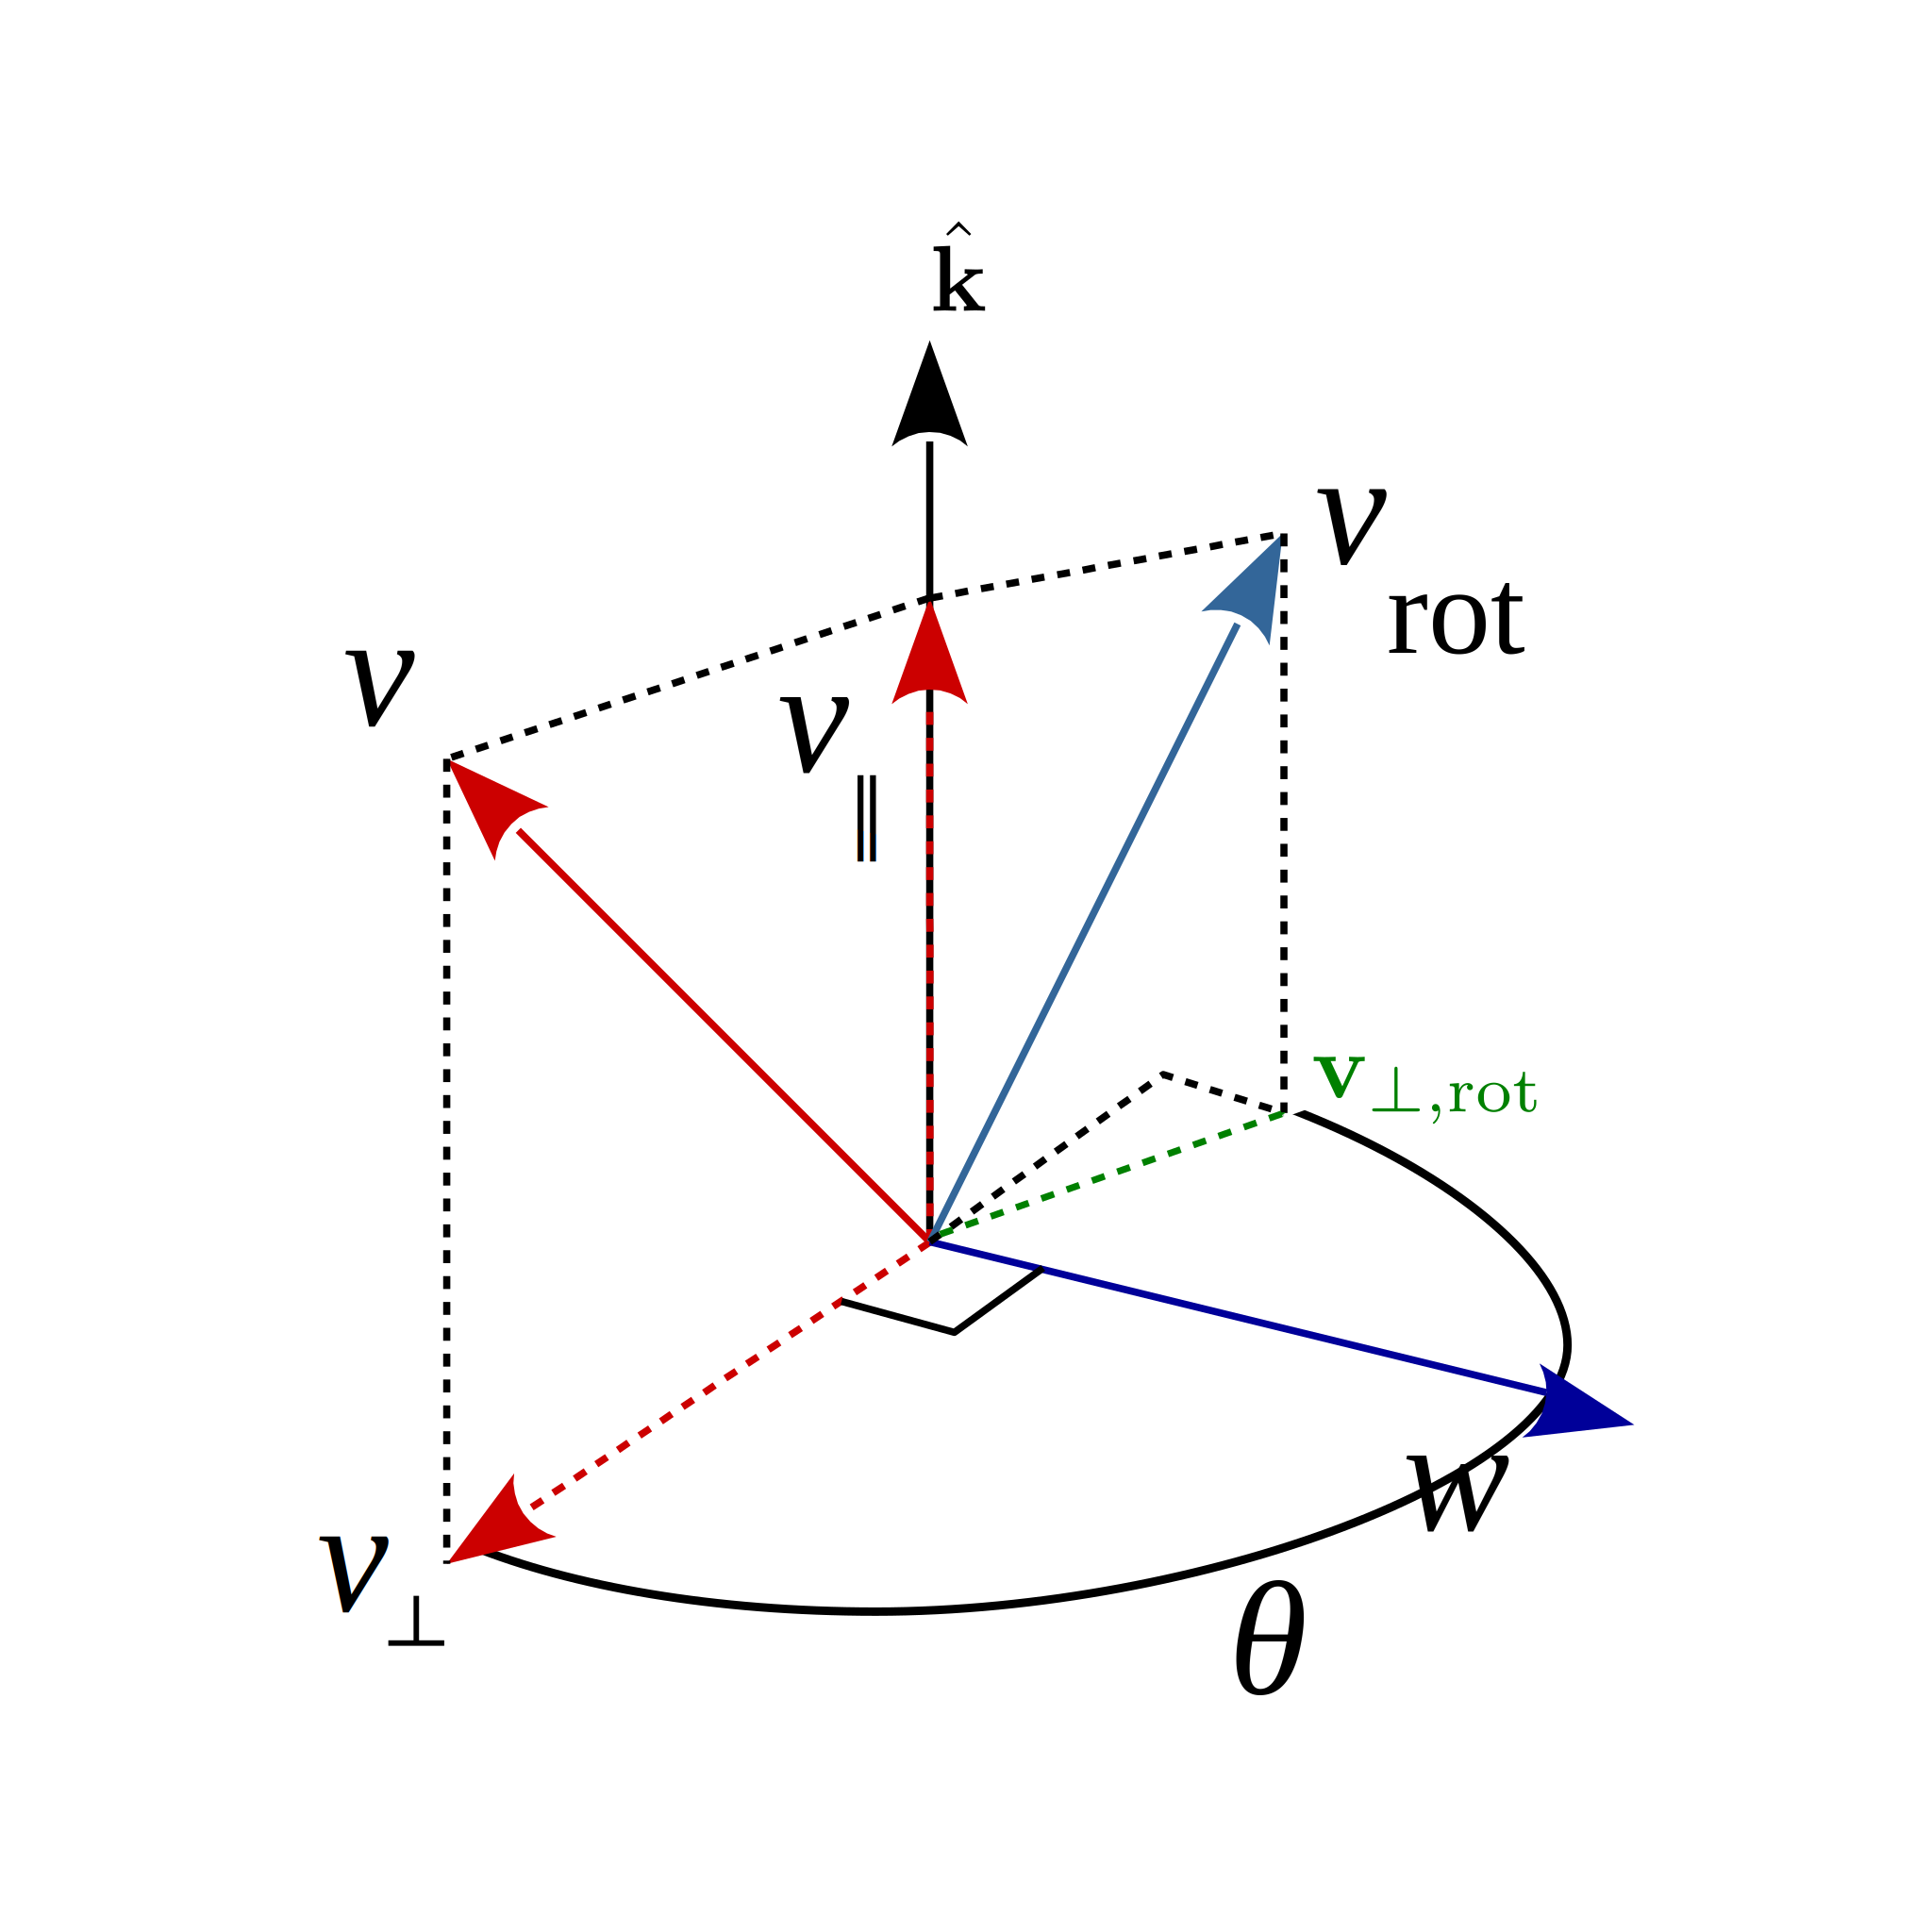
\includegraphics[width=0.5\linewidth]{media/Rodrigues-formula.pdf}
\end{prob}
\begin{solution}
\begin{align}
  \hat{\bfw} = \frac{\hat{\bfk} \times \bfv}{\|\hat{\bfk} \times \bfv\|}
\end{align}
Note that $\hat{\bfk} \times \bfv$ has the magnitude $\|\hat{\bfk} \times \bfv\| = |\hat{\bfk}||\bfv| \sin(\alpha) = |\bfv| \sin(\alpha)$ where $\alpha$ is the angle between $\bfv$ and $\hat{\bfk}$.
\begin{align}
\bfv_\perp = -\hat{\bfk} \times (\hat{\bfk} \times \bfv)
\end{align}
The magnitude of $\bfv_\perp$ is same as RHS because both $|\bfv_\perp| = |\bfv|\sin(\alpha)$ and $|-\hat{\bfk} \times (\hat{\bfk}  \times \bfv)| = |\bfv||\hat{\bfk}|^2 \sin(\alpha) \sin(90^\circ) = |\bfv|\sin(\alpha)$ where $\alpha$ is the angle between $\bfv$ and $\hat{\bfk}$.
\begin{align}
  \bfv_{\perp,rot} = \bfv_\perp \cos(\theta) +
  \hat{\bfw}|\hat{\bfk} \times \bfv| \sin(\theta)
\end{align}
\end{solution}

\newpage

\begin{prob}
  The Euler angles of rotation YZX are given as $\theta$, $\phi$ and $\psi$.
  Derive the rotation matrix corresponding to the Euler angle representation $R = R_x(\psi) R_z(\phi) R_y(\theta)$. Also derive an expression to convert the rotation matrix back to Euler angles. (20 marks).
\end{prob}
\begin{solution}
\begin{align}
  R = R_x(\psi) R_z(\phi) R_y(\theta)
\end{align}
\begin{align}
  \implies \begin{bmatrix}
    r_{11} & r_{12} & r_{13}  \\
    r_{21} & r_{22} & r_{23}  \\
    r_{31} & r_{32} & r_{33}  
  \end{bmatrix}
  =
  \begin{bmatrix}
    1 & 0 & 0\\
    0 & c_\psi & -s_\psi \\
    0 & s_\psi & c_\psi \\
  \end{bmatrix}
  \begin{bmatrix}
    c_\phi & -s_\phi & 0 \\
    s_\phi & c_\phi & 0 \\
    0 & 0 & 1\\
  \end{bmatrix}
  \begin{bmatrix}
    c_\theta & 0 & s_\theta \\
    0 & 1 & 0\\
    -s_\theta & 0 & c_\theta \\
  \end{bmatrix}
\end{align}
\begin{align}
  = \begin{bmatrix}
    1 & 0 & 0\\
    0 & c_\psi & -s_\psi \\
    0 & s_\psi & c_\psi \\
  \end{bmatrix}
  \begin{bmatrix}
    c_\phi c_\theta & - s_\phi & c_\phi s_\theta \\
    s_\phi c_\theta &   c_\phi & s_\phi s_\theta \\
    -s_\theta & 0 & c_\theta \\
  \end{bmatrix}
\end{align}
\begin{align}
  \implies \begin{bmatrix}
    r_{11} & r_{12} & r_{13}  \\
    r_{21} & r_{22} & r_{23}  \\
    r_{31} & r_{32} & r_{33}  
  \end{bmatrix}
  = \begin{bmatrix}
    c_\phi c_\theta & - s_\phi & c_\phi s_\theta \\
    c_\psi s_\phi c_\theta + s_\psi s_\theta &  c_\psi c_\phi & c_\psi s_\phi s_\theta  - s_\psi c_\theta \\
    s_\psi s_\phi c_\theta - c_\psi s_\theta & s_\psi c_\phi & s_\psi s_\phi s_\theta + c_\psi c_\theta
  \end{bmatrix}
\end{align}

\begin{align}
  \phi &= \sin^{-1}(-r_{12}) \in [-\pi/2, \pi/2]\\
  \theta &= \text{arctan2}(r_{13}, r_{11}) \\
  \psi &= \text{arctan2}(r_{32}, r_{22})
\end{align}
\end{solution}
\newpage

\end{document}
